\documentclass{standalone}
\usepackage{tikz}
\usetikzlibrary{patterns, positioning}


\begin{document}
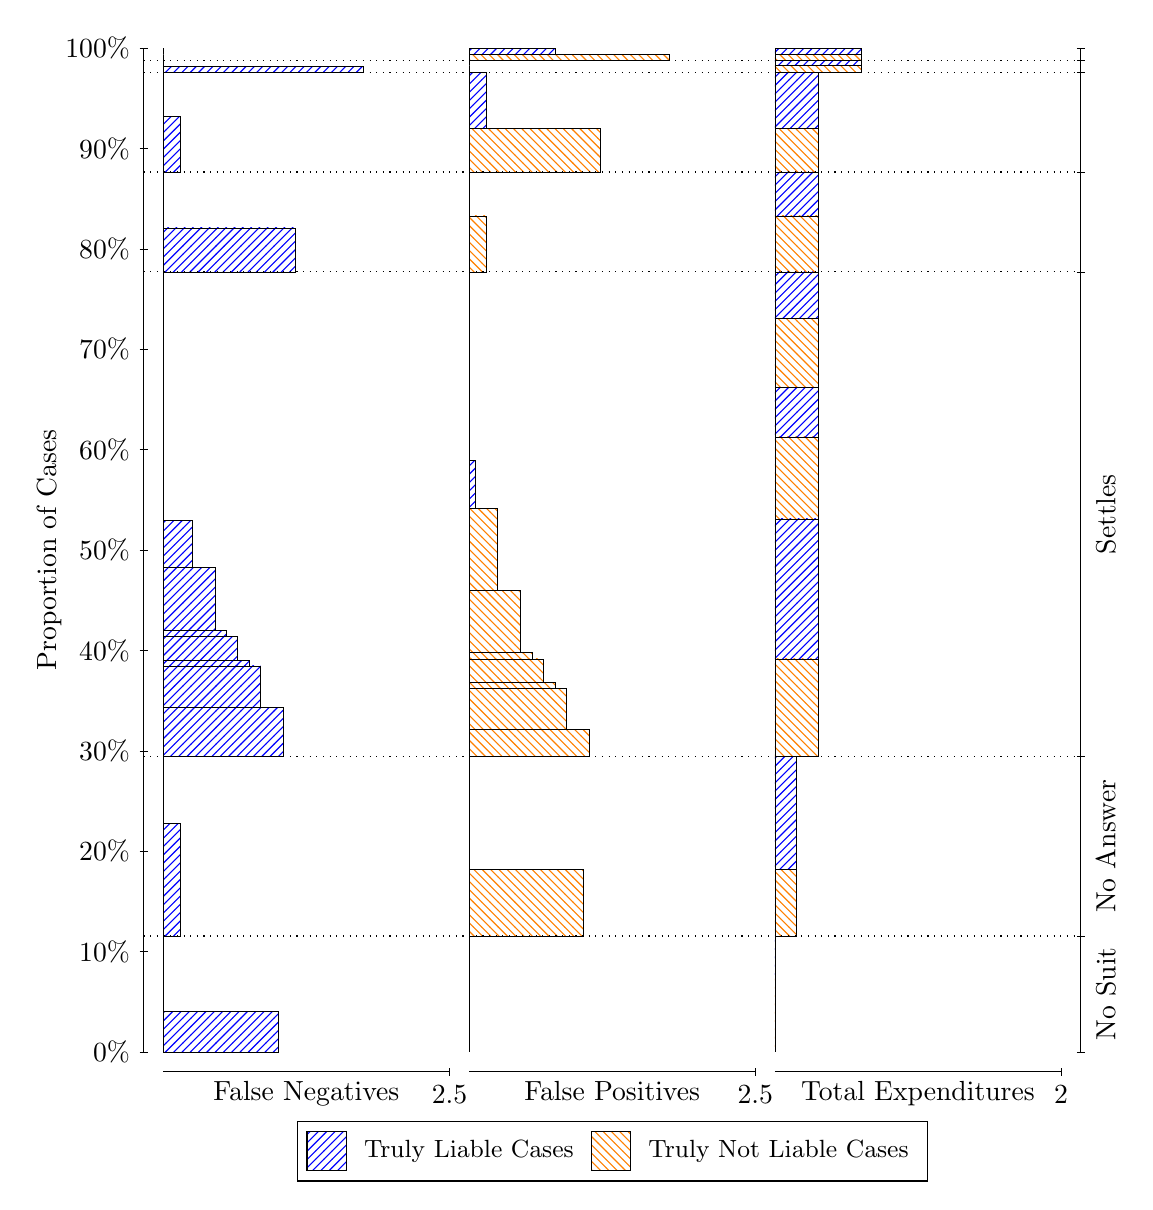
\begin{tikzpicture}
\draw[black, very thin] (1.5,1.75) -- (1.5,14.5);
\node[rotate=90, text=black, anchor=center] at (0.3, 8.125) {Proportion of Cases};
\draw[black, very thin] (1.45,1.75) -- (1.55,1.75);
\node[text=black, anchor=east] at (1.45, 1.75) {0\%};
\draw[black, very thin] (1.45,3.025) -- (1.55,3.025);
\node[text=black, anchor=east] at (1.45, 3.025) {10\%};
\draw[black, very thin] (1.45,4.3) -- (1.55,4.3);
\node[text=black, anchor=east] at (1.45, 4.3) {20\%};
\draw[black, very thin] (1.45,5.575) -- (1.55,5.575);
\node[text=black, anchor=east] at (1.45, 5.575) {30\%};
\draw[black, very thin] (1.45,6.85) -- (1.55,6.85);
\node[text=black, anchor=east] at (1.45, 6.85) {40\%};
\draw[black, very thin] (1.45,8.125) -- (1.55,8.125);
\node[text=black, anchor=east] at (1.45, 8.125) {50\%};
\draw[black, very thin] (1.45,9.4) -- (1.55,9.4);
\node[text=black, anchor=east] at (1.45, 9.4) {60\%};
\draw[black, very thin] (1.45,10.675) -- (1.55,10.675);
\node[text=black, anchor=east] at (1.45, 10.675) {70\%};
\draw[black, very thin] (1.45,11.95) -- (1.55,11.95);
\node[text=black, anchor=east] at (1.45, 11.95) {80\%};
\draw[black, very thin] (1.45,13.225) -- (1.55,13.225);
\node[text=black, anchor=east] at (1.45, 13.225) {90\%};
\draw[black, very thin] (1.45,14.5) -- (1.55,14.5);
\node[text=black, anchor=east] at (1.45, 14.5) {100\%};

\draw[black, very thin] (13.4,1.75) -- (13.4,14.5);
\draw[black, very thin] (13.35,1.75) -- (13.45,1.75);
\node[anchor=west] at (13.35, 1.75) {};
\draw[black, very thin] (13.35,3.2226) -- (13.45,3.2226);
\node[anchor=west] at (13.35, 3.2226) {};
\draw[black, very thin] (13.35,5.5013) -- (13.45,5.5013);
\node[anchor=west] at (13.35, 5.5013) {};
\draw[black, very thin] (13.35,11.657) -- (13.45,11.657);
\node[anchor=west] at (13.35, 11.657) {};
\draw[black, very thin] (13.35,12.926) -- (13.45,12.926);
\node[anchor=west] at (13.35, 12.926) {};
\draw[black, very thin] (13.35,14.194) -- (13.45,14.194);
\node[anchor=west] at (13.35, 14.194) {};
\draw[black, very thin] (13.35,14.347) -- (13.45,14.347);
\node[anchor=west] at (13.35, 14.347) {};
\draw[black, very thin] (13.35,14.5) -- (13.45,14.5);
\node[anchor=west] at (13.35, 14.5) {};

\draw[black, very thin, pattern color=blue, pattern=north east lines] (1.75,1.75) rectangle (3.2033,2.269);
\draw[black, very thin, pattern color=orange, pattern=north west lines] (1.75,2.269) rectangle (1.75,3.2226);
\draw[black, very thin, pattern color=blue, pattern=north east lines] (1.75,3.2226) rectangle (1.968,4.6575);
\draw[black, very thin, pattern color=orange, pattern=north west lines] (1.75,4.6575) rectangle (1.75,5.5013);
\draw[black, very thin, pattern color=blue, pattern=north east lines] (1.75,5.5013) rectangle (3.276,6.1294);
\draw[black, very thin, pattern color=blue, pattern=north east lines] (1.75,6.1294) rectangle (2.9853,6.6525);
\draw[black, very thin, pattern color=blue, pattern=north east lines] (1.75,6.6525) rectangle (2.84,6.7238);
\draw[black, very thin, pattern color=blue, pattern=north east lines] (1.75,6.7238) rectangle (2.6947,7.0268);
\draw[black, very thin, pattern color=blue, pattern=north east lines] (1.75,7.0268) rectangle (2.5493,7.1054);
\draw[black, very thin, pattern color=blue, pattern=north east lines] (1.75,7.1054) rectangle (2.404,7.9001);
\draw[black, very thin, pattern color=blue, pattern=north east lines] (1.75,7.9001) rectangle (2.1133,8.501);
\draw[black, very thin, pattern color=orange, pattern=north west lines] (1.75,8.501) rectangle (1.75,11.657);
\draw[black, very thin, pattern color=blue, pattern=north east lines] (1.75,11.657) rectangle (3.4213,12.216);
\draw[black, very thin, pattern color=orange, pattern=north west lines] (1.75,12.216) rectangle (1.75,12.926);
\draw[black, very thin, pattern color=blue, pattern=north east lines] (1.75,12.926) rectangle (1.968,13.636);
\draw[black, very thin, pattern color=orange, pattern=north west lines] (1.75,13.636) rectangle (1.75,14.194);
\draw[black, very thin, pattern color=blue, pattern=north east lines] (1.75,14.194) rectangle (4.2933,14.263);
\draw[black, very thin, pattern color=orange, pattern=north west lines] (1.75,14.263) rectangle (1.75,14.347);
\draw[black, very thin, pattern color=orange, pattern=north west lines] (1.75,14.347) rectangle (1.75,14.416);
\draw[black, very thin, pattern color=blue, pattern=north east lines] (1.75,14.416) rectangle (1.75,14.5);
\draw[black, very thin, pattern color=orange, pattern=north west lines] (5.6333,1.75) rectangle (5.6333,2.7036);
\draw[black, very thin, pattern color=blue, pattern=north east lines] (5.6333,2.7036) rectangle (5.6333,3.2226);
\draw[black, very thin, pattern color=orange, pattern=north west lines] (5.6333,3.2226) rectangle (7.0867,4.0664);
\draw[black, very thin, pattern color=blue, pattern=north east lines] (5.6333,4.0664) rectangle (5.6333,5.5013);
\draw[black, very thin, pattern color=orange, pattern=north west lines] (5.6333,5.5013) rectangle (7.1593,5.8447);
\draw[black, very thin, pattern color=orange, pattern=north west lines] (5.6333,5.8447) rectangle (6.8687,6.3677);
\draw[black, very thin, pattern color=orange, pattern=north west lines] (5.6333,6.3677) rectangle (6.7233,6.439);
\draw[black, very thin, pattern color=orange, pattern=north west lines] (5.6333,6.439) rectangle (6.578,6.7421);
\draw[black, very thin, pattern color=orange, pattern=north west lines] (5.6333,6.7421) rectangle (6.4327,6.8207);
\draw[black, very thin, pattern color=orange, pattern=north west lines] (5.6333,6.8207) rectangle (6.2873,7.6154);
\draw[black, very thin, pattern color=orange, pattern=north west lines] (5.6333,7.6154) rectangle (5.9967,8.6575);
\draw[black, very thin, pattern color=blue, pattern=north east lines] (5.6333,8.6575) rectangle (5.706,9.2584);
\draw[black, very thin, pattern color=blue, pattern=north east lines] (5.6333,9.2584) rectangle (5.6333,11.657);
\draw[black, very thin, pattern color=orange, pattern=north west lines] (5.6333,11.657) rectangle (5.8513,12.368);
\draw[black, very thin, pattern color=blue, pattern=north east lines] (5.6333,12.368) rectangle (5.6333,12.926);
\draw[black, very thin, pattern color=orange, pattern=north west lines] (5.6333,12.926) rectangle (7.3047,13.484);
\draw[black, very thin, pattern color=blue, pattern=north east lines] (5.6333,13.484) rectangle (5.8513,14.194);
\draw[black, very thin, pattern color=orange, pattern=north west lines] (5.6333,14.194) rectangle (5.6333,14.278);
\draw[black, very thin, pattern color=blue, pattern=north east lines] (5.6333,14.278) rectangle (5.6333,14.347);
\draw[black, very thin, pattern color=orange, pattern=north west lines] (5.6333,14.347) rectangle (8.1767,14.416);
\draw[black, very thin, pattern color=blue, pattern=north east lines] (5.6333,14.416) rectangle (6.7233,14.5);
\draw[black, very thin, pattern color=orange, pattern=north west lines] (9.5167,1.75) rectangle (9.5167,2.7036);
\draw[black, very thin, pattern color=blue, pattern=north east lines] (9.5167,2.7036) rectangle (9.5167,3.2226);
\draw[black, very thin, pattern color=orange, pattern=north west lines] (9.5167,3.2226) rectangle (9.7892,4.0664);
\draw[black, very thin, pattern color=blue, pattern=north east lines] (9.5167,4.0664) rectangle (9.7892,5.5013);
\draw[black, very thin, pattern color=orange, pattern=north west lines] (9.5167,5.5013) rectangle (10.062,6.7421);
\draw[black, very thin, pattern color=blue, pattern=north east lines] (9.5167,6.7421) rectangle (10.062,8.5193);
\draw[black, very thin, pattern color=orange, pattern=north west lines] (9.5167,8.5193) rectangle (10.062,9.5614);
\draw[black, very thin, pattern color=blue, pattern=north east lines] (9.5167,9.5614) rectangle (10.062,10.19);
\draw[black, very thin, pattern color=orange, pattern=north west lines] (9.5167,10.19) rectangle (10.062,11.063);
\draw[black, very thin, pattern color=blue, pattern=north east lines] (9.5167,11.063) rectangle (10.062,11.657);
\draw[black, very thin, pattern color=orange, pattern=north west lines] (9.5167,11.657) rectangle (10.062,12.368);
\draw[black, very thin, pattern color=blue, pattern=north east lines] (9.5167,12.368) rectangle (10.062,12.926);
\draw[black, very thin, pattern color=orange, pattern=north west lines] (9.5167,12.926) rectangle (10.062,13.484);
\draw[black, very thin, pattern color=blue, pattern=north east lines] (9.5167,13.484) rectangle (10.062,14.194);
\draw[black, very thin, pattern color=orange, pattern=north west lines] (9.5167,14.194) rectangle (10.607,14.278);
\draw[black, very thin, pattern color=blue, pattern=north east lines] (9.5167,14.278) rectangle (10.607,14.347);
\draw[black, very thin, pattern color=orange, pattern=north west lines] (9.5167,14.347) rectangle (10.607,14.416);
\draw[black, very thin, pattern color=blue, pattern=north east lines] (9.5167,14.416) rectangle (10.607,14.5);
\draw[black, dotted] (1.5,3.2226) -- (13.4,3.2226);
\draw[black, dotted] (1.5,5.5013) -- (13.4,5.5013);
\draw[black, dotted] (1.5,11.657) -- (13.4,11.657);
\draw[black, dotted] (1.5,12.926) -- (13.4,12.926);
\draw[black, dotted] (1.5,14.194) -- (13.4,14.194);
\draw[black, dotted] (1.5,14.347) -- (13.4,14.347);
\draw[black, very thin] (1.75,1.5) -- (5.3833,1.5);
\node[text=black, anchor=north] at (3.5667, 1.5) {False Negatives};
\draw[black, very thin] (5.3833,1.45) -- (5.3833,1.55);
\node[text=black, anchor=north] at (5.3833, 1.45) {2.5};

\draw[black, very thin] (5.6333,1.5) -- (9.2667,1.5);
\node[text=black, anchor=north] at (7.45, 1.5) {False Positives};
\draw[black, very thin] (9.2667,1.45) -- (9.2667,1.55);
\node[text=black, anchor=north] at (9.2667, 1.45) {2.5};

\draw[black, very thin] (9.5167,1.5) -- (13.15,1.5);
\node[text=black, anchor=north] at (11.333, 1.5) {Total Expenditures};
\draw[black, very thin] (13.15,1.45) -- (13.15,1.55);
\node[text=black, anchor=north] at (13.15, 1.45) {2};

\node[text=black, centered, rotate=90] at (13.72, 2.4863) {No Suit};
\node[text=black, centered, rotate=90] at (13.72, 4.362) {No Answer};
\node[text=black, centered, rotate=90] at (13.72, 8.5793) {Settles};





\draw (7.449999999999999,1.5) node[draw=none] (baseCoordinate) {};
\begin{scope}[align=center]
        \matrix[scale=0.5, draw=black, below=0.5cm of baseCoordinate, nodes={draw}, column sep=0.1cm]{
            \node[rectangle, draw, minimum width=0.5cm, minimum height=0.5cm, pattern color=blue, pattern=north east lines] {}; &
            \node[draw=none, font=\small, text=black] (B) {Truly Liable Cases}; &
            \node[rectangle, draw, minimum width=0.5cm, minimum height=0.5cm, pattern color=orange, pattern=north west lines] {}; &
            \node[draw=none, font=\small, text=black] (B) {Truly Not Liable Cases}; \\
            };
\end{scope}

\end{tikzpicture}
\end{document}